\documentclass{standalone}
\usepackage{tikz}
\usetikzlibrary{patterns, positioning}
\usepackage[sfdefault]{ClearSans} %% option 'sfdefault' activates Clear Sans as the default text font
\usepackage[T1]{fontenc}

\begin{document}
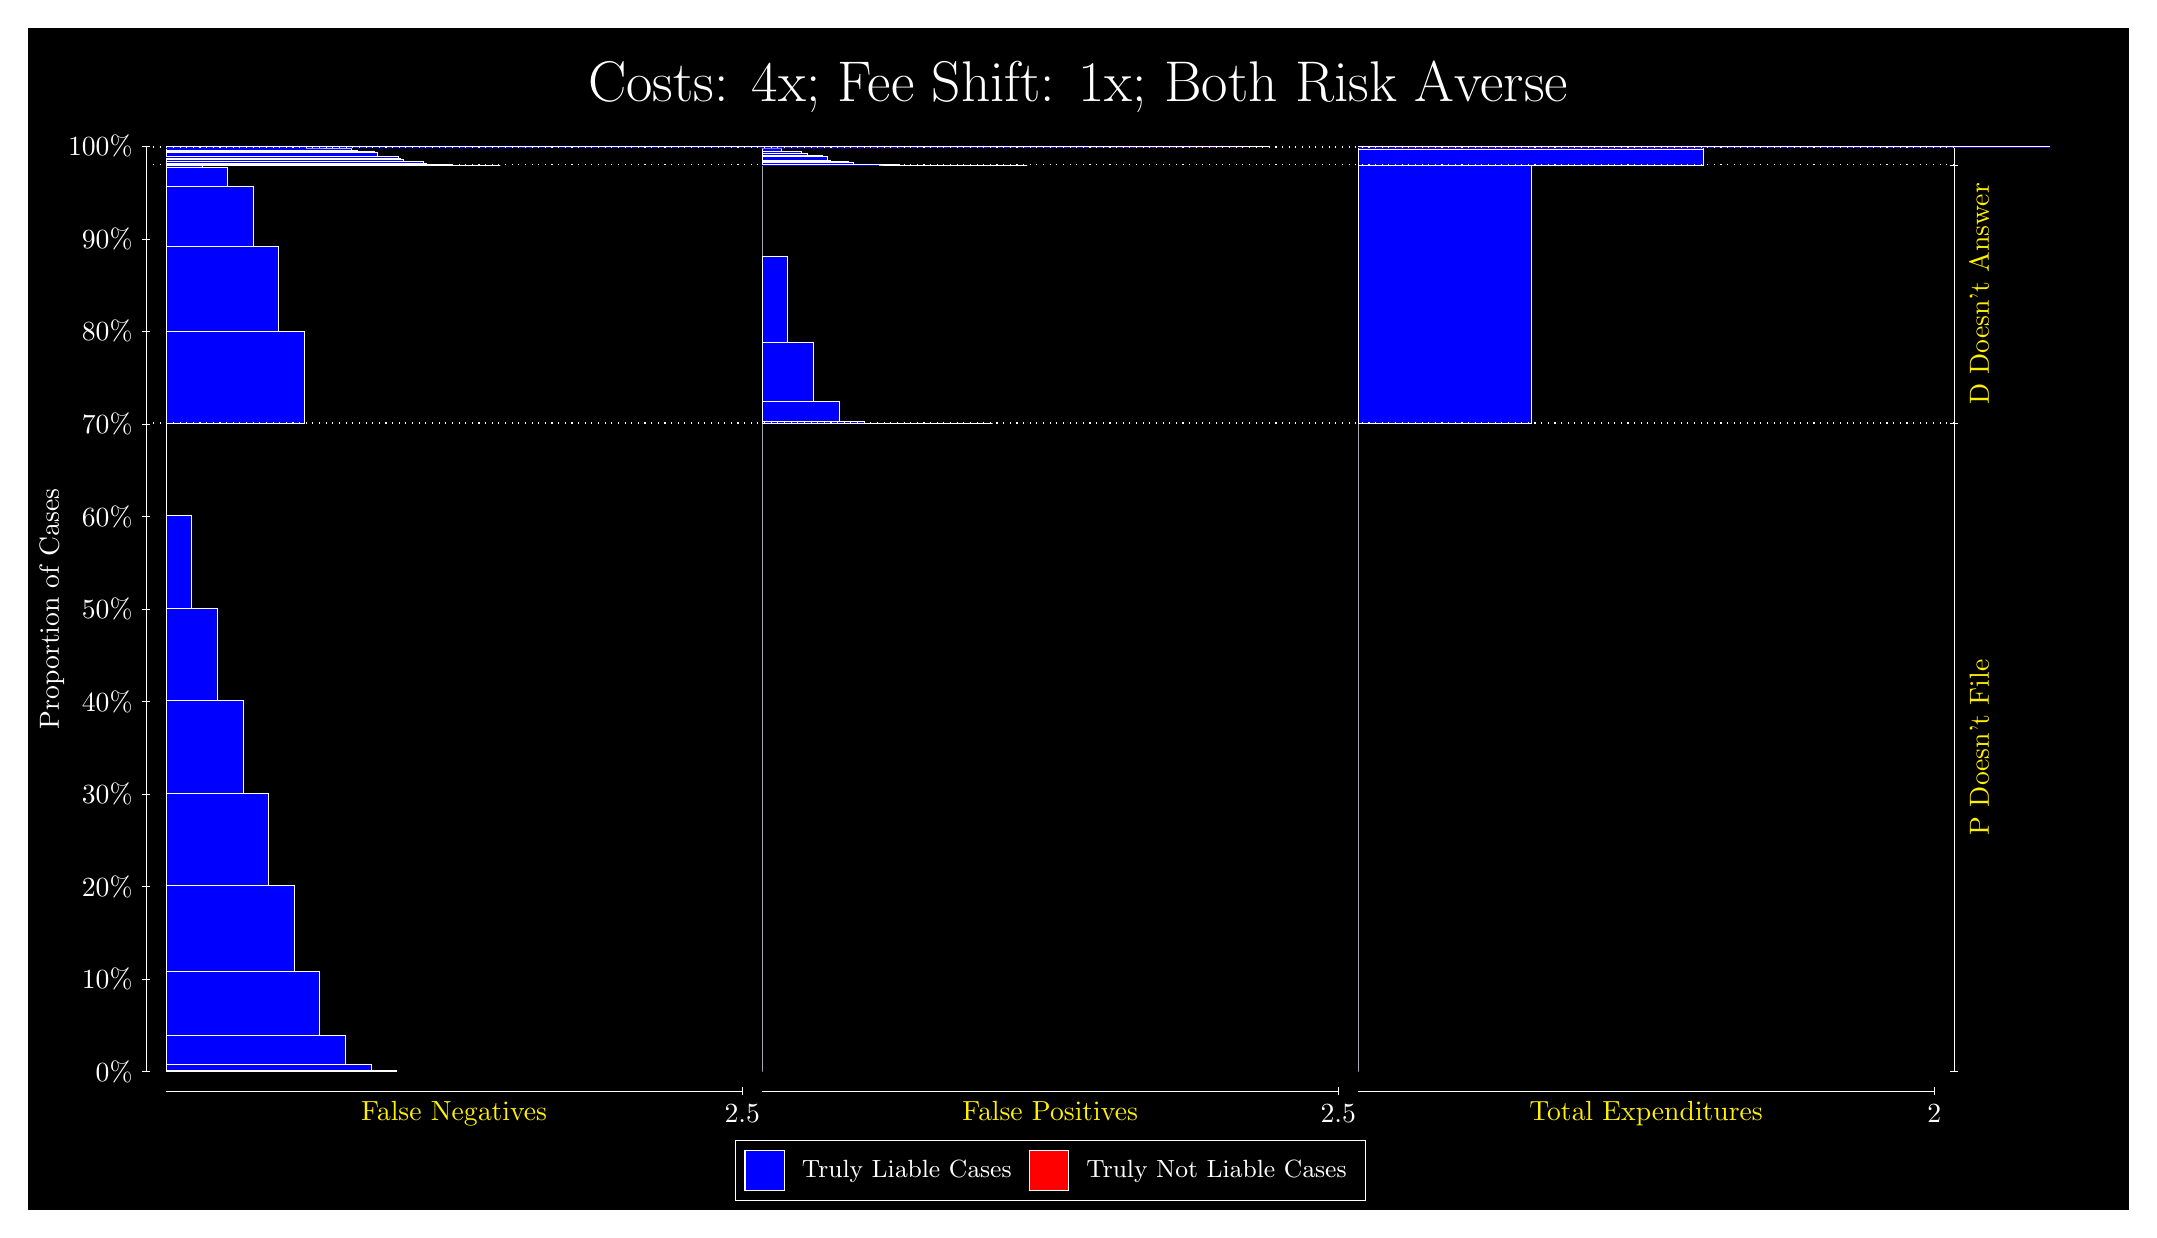
\begin{tikzpicture}
\draw[fill=black] (0,0) rectangle (26.667,15);
\draw[text=white] (0,13.5) rectangle (26.667,15) node[midway] {\huge Costs: 4x; Fee Shift: 1x; Both Risk Averse};
\draw[white, very thin] (1.5,1.75) -- (1.5,13.5);
\node[rotate=90, text=white, anchor=center] at (0.3, 7.625) {Proportion of Cases};
\draw[white, very thin] (1.45,1.75) -- (1.55,1.75);
\node[text=white, anchor=east] at (1.45, 1.75) {0\%};
\draw[white, very thin] (1.45,2.925) -- (1.55,2.925);
\node[text=white, anchor=east] at (1.45, 2.925) {10\%};
\draw[white, very thin] (1.45,4.1) -- (1.55,4.1);
\node[text=white, anchor=east] at (1.45, 4.1) {20\%};
\draw[white, very thin] (1.45,5.275) -- (1.55,5.275);
\node[text=white, anchor=east] at (1.45, 5.275) {30\%};
\draw[white, very thin] (1.45,6.45) -- (1.55,6.45);
\node[text=white, anchor=east] at (1.45, 6.45) {40\%};
\draw[white, very thin] (1.45,7.625) -- (1.55,7.625);
\node[text=white, anchor=east] at (1.45, 7.625) {50\%};
\draw[white, very thin] (1.45,8.8) -- (1.55,8.8);
\node[text=white, anchor=east] at (1.45, 8.8) {60\%};
\draw[white, very thin] (1.45,9.975) -- (1.55,9.975);
\node[text=white, anchor=east] at (1.45, 9.975) {70\%};
\draw[white, very thin] (1.45,11.15) -- (1.55,11.15);
\node[text=white, anchor=east] at (1.45, 11.15) {80\%};
\draw[white, very thin] (1.45,12.325) -- (1.55,12.325);
\node[text=white, anchor=east] at (1.45, 12.325) {90\%};
\draw[white, very thin] (1.45,13.5) -- (1.55,13.5);
\node[text=white, anchor=east] at (1.45, 13.5) {100\%};

\draw[white, very thin] (24.457,1.75) -- (24.457,13.5);
\draw[white, very thin] (24.407,1.75) -- (24.507,1.75);
\node[anchor=west] at (24.407, 1.75) {};
\draw[white, very thin] (24.407,9.986) -- (24.507,9.986);
\node[anchor=west] at (24.407, 9.986) {};
\draw[white, very thin] (24.407,13.265) -- (24.507,13.265);
\node[anchor=west] at (24.407, 13.265) {};
\draw[white, very thin] (24.407,13.484) -- (24.507,13.484);
\node[anchor=west] at (24.407, 13.484) {};
\draw[white, very thin] (24.407,13.496) -- (24.507,13.496);
\node[anchor=west] at (24.407, 13.496) {};
\draw[white, very thin] (24.407,13.496) -- (24.507,13.496);
\node[anchor=west] at (24.407, 13.496) {};
\draw[white, very thin] (24.407,13.5) -- (24.507,13.5);
\node[anchor=west] at (24.407, 13.5) {};

\draw[white, very thin, fill=blue] (1.75,1.75) rectangle (4.6775,1.7606);
\draw[white, very thin, fill=blue] (1.75,1.7606) rectangle (4.3523,1.8447);
\draw[white, very thin, fill=blue] (1.75,1.8447) rectangle (4.027,2.2095);
\draw[white, very thin, fill=blue] (1.75,2.2095) rectangle (3.7017,3.0221);
\draw[white, very thin, fill=blue] (1.75,3.0221) rectangle (3.3764,4.1186);
\draw[white, very thin, fill=blue] (1.75,4.1186) rectangle (3.0511,5.2863);
\draw[white, very thin, fill=blue] (1.75,5.2863) rectangle (2.7258,6.4611);
\draw[white, very thin, fill=blue] (1.75,6.4611) rectangle (2.4006,7.636);
\draw[white, very thin, fill=blue] (1.75,7.636) rectangle (2.0753,8.8111);
\draw[white, very thin, fill=red] (1.75,8.8111) rectangle (1.75,8.8111);
\draw[white, very thin, fill=blue] (1.75,8.8111) rectangle (1.75,9.986);
\draw[white, very thin, fill=blue] (1.75,9.986) rectangle (3.5065,11.15);
\draw[white, very thin, fill=blue] (1.75,11.15) rectangle (3.1812,12.234);
\draw[white, very thin, fill=blue] (1.75,12.234) rectangle (2.856,12.989);
\draw[white, very thin, fill=blue] (1.75,12.989) rectangle (2.5307,13.24);
\draw[white, very thin, fill=blue] (1.75,13.24) rectangle (2.2054,13.264);
\draw[white, very thin, fill=blue] (1.75,13.264) rectangle (1.8801,13.265);
\draw[white, very thin, fill=red] (1.75,13.265) rectangle (1.75,13.265);
\draw[white, very thin, fill=blue] (1.75,13.265) rectangle (1.75,13.265);
\draw[white, very thin, fill=blue] (1.75,13.265) rectangle (5.9949,13.265);
\draw[white, very thin, fill=blue] (1.75,13.265) rectangle (5.7022,13.265);
\draw[white, very thin, fill=blue] (1.75,13.265) rectangle (5.6697,13.265);
\draw[white, very thin, fill=blue] (1.75,13.265) rectangle (5.4094,13.265);
\draw[white, very thin, fill=blue] (1.75,13.265) rectangle (5.3769,13.266);
\draw[white, very thin, fill=blue] (1.75,13.266) rectangle (5.3444,13.272);
\draw[white, very thin, fill=blue] (1.75,13.272) rectangle (5.1167,13.272);
\draw[white, very thin, fill=blue] (1.75,13.272) rectangle (5.0842,13.275);
\draw[white, very thin, fill=blue] (1.75,13.275) rectangle (5.0516,13.279);
\draw[white, very thin, fill=blue] (1.75,13.279) rectangle (5.0191,13.307);
\draw[white, very thin, fill=blue] (1.75,13.307) rectangle (4.8239,13.307);
\draw[white, very thin, fill=blue] (1.75,13.307) rectangle (4.7914,13.308);
\draw[white, very thin, fill=blue] (1.75,13.308) rectangle (4.7589,13.333);
\draw[white, very thin, fill=blue] (1.75,13.333) rectangle (4.7263,13.342);
\draw[white, very thin, fill=blue] (1.75,13.342) rectangle (4.6938,13.368);
\draw[white, very thin, fill=blue] (1.75,13.368) rectangle (4.4986,13.37);
\draw[white, very thin, fill=blue] (1.75,13.37) rectangle (4.4661,13.374);
\draw[white, very thin, fill=blue] (1.75,13.374) rectangle (4.4336,13.375);
\draw[white, very thin, fill=blue] (1.75,13.375) rectangle (4.4336,13.43);
\draw[white, very thin, fill=blue] (1.75,13.43) rectangle (4.4011,13.433);
\draw[white, very thin, fill=blue] (1.75,13.433) rectangle (4.3685,13.439);
\draw[white, very thin, fill=blue] (1.75,13.439) rectangle (4.1734,13.448);
\draw[white, very thin, fill=blue] (1.75,13.448) rectangle (4.1408,13.452);
\draw[white, very thin, fill=blue] (1.75,13.452) rectangle (4.1083,13.473);
\draw[white, very thin, fill=blue] (1.75,13.473) rectangle (4.0758,13.473);
\draw[white, very thin, fill=blue] (1.75,13.473) rectangle (4.0432,13.473);
\draw[white, very thin, fill=blue] (1.75,13.473) rectangle (3.8481,13.481);
\draw[white, very thin, fill=blue] (1.75,13.481) rectangle (3.8155,13.481);
\draw[white, very thin, fill=blue] (1.75,13.481) rectangle (3.783,13.483);
\draw[white, very thin, fill=blue] (1.75,13.483) rectangle (3.7505,13.483);
\draw[white, very thin, fill=blue] (1.75,13.483) rectangle (3.718,13.483);
\draw[white, very thin, fill=blue] (1.75,13.483) rectangle (3.5228,13.484);
\draw[white, very thin, fill=blue] (1.75,13.484) rectangle (3.4903,13.484);
\draw[white, very thin, fill=blue] (1.75,13.484) rectangle (3.4577,13.484);
\draw[white, very thin, fill=blue] (1.75,13.484) rectangle (3.4252,13.484);
\draw[white, very thin, fill=blue] (1.75,13.484) rectangle (3.3927,13.484);
\draw[white, very thin, fill=blue] (1.75,13.484) rectangle (3.1975,13.484);
\draw[white, very thin, fill=blue] (1.75,13.484) rectangle (3.165,13.484);
\draw[white, very thin, fill=blue] (1.75,13.484) rectangle (3.1325,13.484);
\draw[white, very thin, fill=blue] (1.75,13.484) rectangle (3.1325,13.484);
\draw[white, very thin, fill=blue] (1.75,13.484) rectangle (3.0999,13.484);
\draw[white, very thin, fill=blue] (1.75,13.484) rectangle (3.0674,13.484);
\draw[white, very thin, fill=blue] (1.75,13.484) rectangle (2.8722,13.484);
\draw[white, very thin, fill=blue] (1.75,13.484) rectangle (2.8397,13.484);
\draw[white, very thin, fill=blue] (1.75,13.484) rectangle (2.8072,13.484);
\draw[white, very thin, fill=blue] (1.75,13.484) rectangle (2.8072,13.484);
\draw[white, very thin, fill=blue] (1.75,13.484) rectangle (2.7746,13.484);
\draw[white, very thin, fill=blue] (1.75,13.484) rectangle (2.5469,13.484);
\draw[white, very thin, fill=blue] (1.75,13.484) rectangle (2.5144,13.484);
\draw[white, very thin, fill=blue] (1.75,13.484) rectangle (2.4819,13.484);
\draw[white, very thin, fill=blue] (1.75,13.484) rectangle (2.4819,13.484);
\draw[white, very thin, fill=blue] (1.75,13.484) rectangle (2.2217,13.484);
\draw[white, very thin, fill=blue] (1.75,13.484) rectangle (2.1891,13.484);
\draw[white, very thin, fill=blue] (1.75,13.484) rectangle (1.8964,13.484);
\draw[white, very thin, fill=red] (1.75,13.484) rectangle (1.75,13.484);
\draw[white, very thin, fill=blue] (1.75,13.484) rectangle (6.4341,13.484);
\draw[white, very thin, fill=blue] (1.75,13.484) rectangle (6.1088,13.484);
\draw[white, very thin, fill=blue] (1.75,13.484) rectangle (5.7835,13.488);
\draw[white, very thin, fill=blue] (1.75,13.488) rectangle (5.4582,13.494);
\draw[white, very thin, fill=blue] (1.75,13.494) rectangle (5.1329,13.496);
\draw[white, very thin, fill=blue] (1.75,13.496) rectangle (4.8077,13.496);
\draw[white, very thin, fill=blue] (1.75,13.496) rectangle (4.4824,13.496);
\draw[white, very thin, fill=blue] (1.75,13.496) rectangle (4.1571,13.496);
\draw[white, very thin, fill=blue] (1.75,13.496) rectangle (3.8318,13.496);
\draw[white, very thin, fill=blue] (1.75,13.496) rectangle (3.5065,13.496);
\draw[white, very thin, fill=red] (1.75,13.496) rectangle (1.75,13.496);
\draw[white, very thin, fill=blue] (1.75,13.496) rectangle (3.5065,13.496);
\draw[white, very thin, fill=blue] (1.75,13.496) rectangle (3.1812,13.496);
\draw[white, very thin, fill=blue] (1.75,13.496) rectangle (2.856,13.496);
\draw[white, very thin, fill=blue] (1.75,13.496) rectangle (2.5307,13.496);
\draw[white, very thin, fill=blue] (1.75,13.496) rectangle (2.2054,13.496);
\draw[white, very thin, fill=blue] (1.75,13.496) rectangle (1.8801,13.496);
\draw[white, very thin, fill=red] (1.75,13.496) rectangle (1.75,13.496);
\draw[white, very thin, fill=blue] (1.75,13.496) rectangle (1.75,13.496);
\draw[white, very thin, fill=blue] (1.75,13.496) rectangle (11.704,13.496);
\draw[white, very thin, fill=blue] (1.75,13.496) rectangle (11.378,13.496);
\draw[white, very thin, fill=blue] (1.75,13.496) rectangle (11.053,13.496);
\draw[white, very thin, fill=blue] (1.75,13.496) rectangle (10.728,13.496);
\draw[white, very thin, fill=blue] (1.75,13.496) rectangle (10.403,13.496);
\draw[white, very thin, fill=blue] (1.75,13.496) rectangle (10.403,13.496);
\draw[white, very thin, fill=blue] (1.75,13.496) rectangle (10.077,13.496);
\draw[white, very thin, fill=blue] (1.75,13.496) rectangle (9.752,13.496);
\draw[white, very thin, fill=blue] (1.75,13.496) rectangle (9.752,13.496);
\draw[white, very thin, fill=blue] (1.75,13.496) rectangle (9.4267,13.496);
\draw[white, very thin, fill=blue] (1.75,13.496) rectangle (9.4267,13.496);
\draw[white, very thin, fill=blue] (1.75,13.496) rectangle (9.1014,13.496);
\draw[white, very thin, fill=blue] (1.75,13.496) rectangle (8.7761,13.496);
\draw[white, very thin, fill=blue] (1.75,13.496) rectangle (8.4508,13.496);
\draw[white, very thin, fill=blue] (1.75,13.496) rectangle (8.1255,13.496);
\draw[white, very thin, fill=blue] (1.75,13.496) rectangle (7.8003,13.496);
\draw[white, very thin, fill=blue] (1.75,13.496) rectangle (7.54,13.496);
\draw[white, very thin, fill=blue] (1.75,13.496) rectangle (7.2148,13.496);
\draw[white, very thin, fill=blue] (1.75,13.496) rectangle (6.8895,13.496);
\draw[white, very thin, fill=blue] (1.75,13.496) rectangle (6.5642,13.496);
\draw[white, very thin, fill=blue] (1.75,13.496) rectangle (6.2389,13.497);
\draw[white, very thin, fill=blue] (1.75,13.497) rectangle (5.9136,13.497);
\draw[white, very thin, fill=blue] (1.75,13.497) rectangle (5.9136,13.497);
\draw[white, very thin, fill=blue] (1.75,13.497) rectangle (5.5883,13.497);
\draw[white, very thin, fill=blue] (1.75,13.497) rectangle (5.5883,13.498);
\draw[white, very thin, fill=blue] (1.75,13.498) rectangle (5.2631,13.499);
\draw[white, very thin, fill=blue] (1.75,13.499) rectangle (4.9378,13.499);
\draw[white, very thin, fill=blue] (1.75,13.499) rectangle (4.9378,13.5);
\draw[white, very thin, fill=blue] (1.75,13.5) rectangle (4.6125,13.5);
\draw[white, very thin, fill=blue] (1.75,13.5) rectangle (4.6125,13.5);
\draw[white, very thin, fill=blue] (1.75,13.5) rectangle (4.6125,13.5);
\draw[white, very thin, fill=blue] (1.75,13.5) rectangle (4.2872,13.5);
\draw[white, very thin, fill=blue] (1.75,13.5) rectangle (4.2872,13.5);
\draw[white, very thin, fill=blue] (1.75,13.5) rectangle (3.9619,13.5);
\draw[white, very thin, fill=blue] (1.75,13.5) rectangle (3.6366,13.5);
\draw[white, very thin, fill=blue] (1.75,13.5) rectangle (3.3114,13.5);
\draw[white, very thin, fill=blue] (1.75,13.5) rectangle (3.3114,13.5);
\draw[white, very thin, fill=blue] (1.75,13.5) rectangle (2.9861,13.5);
\draw[white, very thin, fill=blue] (1.75,13.5) rectangle (2.9861,13.5);
\draw[white, very thin, fill=blue] (1.75,13.5) rectangle (2.6608,13.5);
\draw[white, very thin, fill=blue] (1.75,13.5) rectangle (2.6608,13.5);
\draw[white, very thin, fill=blue] (1.75,13.5) rectangle (2.3355,13.5);
\draw[white, very thin, fill=red] (1.75,13.5) rectangle (1.75,13.5);
\draw[white, very thin, fill=red] (9.3189,1.75) rectangle (9.3189,1.75);
\draw[white, very thin, fill=blue] (9.3189,1.75) rectangle (9.3189,9.986);
\draw[white, very thin, fill=red] (9.3189,9.986) rectangle (12.246,9.986);
\draw[white, very thin, fill=blue] (9.3189,9.986) rectangle (12.246,9.986);
\draw[white, very thin, fill=blue] (9.3189,9.986) rectangle (11.921,9.986);
\draw[white, very thin, fill=blue] (9.3189,9.986) rectangle (11.596,9.986);
\draw[white, very thin, fill=blue] (9.3189,9.986) rectangle (11.271,9.986);
\draw[white, very thin, fill=blue] (9.3189,9.986) rectangle (10.945,9.9865);
\draw[white, very thin, fill=blue] (9.3189,9.9865) rectangle (10.62,10.011);
\draw[white, very thin, fill=blue] (9.3189,10.011) rectangle (10.295,10.261);
\draw[white, very thin, fill=blue] (9.3189,10.261) rectangle (9.9694,11.017);
\draw[white, very thin, fill=blue] (9.3189,11.017) rectangle (9.6442,12.101);
\draw[white, very thin, fill=blue] (9.3189,12.101) rectangle (9.3189,13.265);
\draw[white, very thin, fill=red] (9.3189,13.265) rectangle (12.686,13.265);
\draw[white, very thin, fill=blue] (9.3189,13.265) rectangle (12.686,13.265);
\draw[white, very thin, fill=red] (9.3189,13.265) rectangle (12.393,13.265);
\draw[white, very thin, fill=blue] (9.3189,13.265) rectangle (12.393,13.265);
\draw[white, very thin, fill=blue] (9.3189,13.265) rectangle (12.36,13.265);
\draw[white, very thin, fill=red] (9.3189,13.265) rectangle (12.1,13.265);
\draw[white, very thin, fill=blue] (9.3189,13.265) rectangle (12.1,13.265);
\draw[white, very thin, fill=blue] (9.3189,13.265) rectangle (12.068,13.265);
\draw[white, very thin, fill=blue] (9.3189,13.265) rectangle (12.035,13.265);
\draw[white, very thin, fill=red] (9.3189,13.265) rectangle (11.807,13.265);
\draw[white, very thin, fill=blue] (9.3189,13.265) rectangle (11.807,13.265);
\draw[white, very thin, fill=blue] (9.3189,13.265) rectangle (11.775,13.265);
\draw[white, very thin, fill=blue] (9.3189,13.265) rectangle (11.742,13.265);
\draw[white, very thin, fill=blue] (9.3189,13.265) rectangle (11.71,13.265);
\draw[white, very thin, fill=red] (9.3189,13.265) rectangle (11.515,13.265);
\draw[white, very thin, fill=blue] (9.3189,13.265) rectangle (11.515,13.265);
\draw[white, very thin, fill=blue] (9.3189,13.265) rectangle (11.482,13.265);
\draw[white, very thin, fill=blue] (9.3189,13.265) rectangle (11.449,13.265);
\draw[white, very thin, fill=blue] (9.3189,13.265) rectangle (11.417,13.265);
\draw[white, very thin, fill=blue] (9.3189,13.265) rectangle (11.384,13.265);
\draw[white, very thin, fill=blue] (9.3189,13.265) rectangle (11.189,13.265);
\draw[white, very thin, fill=blue] (9.3189,13.265) rectangle (11.157,13.265);
\draw[white, very thin, fill=blue] (9.3189,13.265) rectangle (11.124,13.265);
\draw[white, very thin, fill=blue] (9.3189,13.265) rectangle (11.092,13.265);
\draw[white, very thin, fill=blue] (9.3189,13.265) rectangle (11.059,13.266);
\draw[white, very thin, fill=blue] (9.3189,13.266) rectangle (10.864,13.266);
\draw[white, very thin, fill=blue] (9.3189,13.266) rectangle (10.831,13.266);
\draw[white, very thin, fill=blue] (9.3189,13.266) rectangle (10.799,13.267);
\draw[white, very thin, fill=blue] (9.3189,13.267) rectangle (10.766,13.268);
\draw[white, very thin, fill=blue] (9.3189,13.268) rectangle (10.734,13.275);
\draw[white, very thin, fill=blue] (9.3189,13.275) rectangle (10.539,13.275);
\draw[white, very thin, fill=blue] (9.3189,13.275) rectangle (10.506,13.276);
\draw[white, very thin, fill=blue] (9.3189,13.276) rectangle (10.474,13.297);
\draw[white, very thin, fill=blue] (9.3189,13.297) rectangle (10.441,13.301);
\draw[white, very thin, fill=blue] (9.3189,13.301) rectangle (10.409,13.31);
\draw[white, very thin, fill=blue] (9.3189,13.31) rectangle (10.213,13.315);
\draw[white, very thin, fill=blue] (9.3189,13.315) rectangle (10.181,13.319);
\draw[white, very thin, fill=blue] (9.3189,13.319) rectangle (10.148,13.374);
\draw[white, very thin, fill=blue] (9.3189,13.374) rectangle (10.116,13.379);
\draw[white, very thin, fill=blue] (9.3189,13.379) rectangle (10.083,13.381);
\draw[white, very thin, fill=blue] (9.3189,13.381) rectangle (9.8881,13.407);
\draw[white, very thin, fill=blue] (9.3189,13.407) rectangle (9.8556,13.416);
\draw[white, very thin, fill=blue] (9.3189,13.416) rectangle (9.8231,13.441);
\draw[white, very thin, fill=blue] (9.3189,13.441) rectangle (9.7905,13.441);
\draw[white, very thin, fill=blue] (9.3189,13.441) rectangle (9.758,13.442);
\draw[white, very thin, fill=blue] (9.3189,13.442) rectangle (9.5628,13.47);
\draw[white, very thin, fill=blue] (9.3189,13.47) rectangle (9.5303,13.474);
\draw[white, very thin, fill=blue] (9.3189,13.474) rectangle (9.4978,13.476);
\draw[white, very thin, fill=blue] (9.3189,13.476) rectangle (9.4652,13.476);
\draw[white, very thin, fill=blue] (9.3189,13.476) rectangle (9.3189,13.484);
\draw[white, very thin, fill=red] (9.3189,13.484) rectangle (11.075,13.484);
\draw[white, very thin, fill=blue] (9.3189,13.484) rectangle (11.075,13.484);
\draw[white, very thin, fill=blue] (9.3189,13.484) rectangle (10.75,13.484);
\draw[white, very thin, fill=blue] (9.3189,13.484) rectangle (10.425,13.484);
\draw[white, very thin, fill=blue] (9.3189,13.484) rectangle (10.1,13.484);
\draw[white, very thin, fill=blue] (9.3189,13.484) rectangle (9.7743,13.484);
\draw[white, very thin, fill=blue] (9.3189,13.484) rectangle (9.449,13.486);
\draw[white, very thin, fill=blue] (9.3189,13.486) rectangle (9.3189,13.496);
\draw[white, very thin, fill=red] (9.3189,13.496) rectangle (14.003,13.496);
\draw[white, very thin, fill=blue] (9.3189,13.496) rectangle (14.003,13.496);
\draw[white, very thin, fill=blue] (9.3189,13.496) rectangle (13.678,13.496);
\draw[white, very thin, fill=blue] (9.3189,13.496) rectangle (13.352,13.496);
\draw[white, very thin, fill=blue] (9.3189,13.496) rectangle (13.027,13.496);
\draw[white, very thin, fill=blue] (9.3189,13.496) rectangle (12.702,13.496);
\draw[white, very thin, fill=blue] (9.3189,13.496) rectangle (12.377,13.496);
\draw[white, very thin, fill=blue] (9.3189,13.496) rectangle (12.051,13.496);
\draw[white, very thin, fill=blue] (9.3189,13.496) rectangle (11.726,13.496);
\draw[white, very thin, fill=blue] (9.3189,13.496) rectangle (11.401,13.496);
\draw[white, very thin, fill=blue] (9.3189,13.496) rectangle (11.075,13.496);
\draw[white, very thin, fill=red] (9.3189,13.496) rectangle (15.759,13.496);
\draw[white, very thin, fill=blue] (9.3189,13.496) rectangle (15.759,13.496);
\draw[white, very thin, fill=blue] (9.3189,13.496) rectangle (15.434,13.496);
\draw[white, very thin, fill=red] (9.3189,13.496) rectangle (15.434,13.496);
\draw[white, very thin, fill=blue] (9.3189,13.496) rectangle (15.434,13.496);
\draw[white, very thin, fill=red] (9.3189,13.496) rectangle (15.109,13.496);
\draw[white, very thin, fill=blue] (9.3189,13.496) rectangle (15.109,13.496);
\draw[white, very thin, fill=blue] (9.3189,13.496) rectangle (15.109,13.496);
\draw[white, very thin, fill=blue] (9.3189,13.496) rectangle (14.784,13.496);
\draw[white, very thin, fill=red] (9.3189,13.496) rectangle (14.784,13.496);
\draw[white, very thin, fill=blue] (9.3189,13.496) rectangle (14.784,13.496);
\draw[white, very thin, fill=blue] (9.3189,13.496) rectangle (14.784,13.496);
\draw[white, very thin, fill=blue] (9.3189,13.496) rectangle (14.458,13.496);
\draw[white, very thin, fill=red] (9.3189,13.496) rectangle (14.458,13.496);
\draw[white, very thin, fill=blue] (9.3189,13.496) rectangle (14.458,13.496);
\draw[white, very thin, fill=blue] (9.3189,13.496) rectangle (14.458,13.496);
\draw[white, very thin, fill=blue] (9.3189,13.496) rectangle (14.133,13.496);
\draw[white, very thin, fill=red] (9.3189,13.496) rectangle (14.133,13.496);
\draw[white, very thin, fill=blue] (9.3189,13.496) rectangle (14.133,13.496);
\draw[white, very thin, fill=blue] (9.3189,13.496) rectangle (14.133,13.496);
\draw[white, very thin, fill=blue] (9.3189,13.496) rectangle (13.808,13.496);
\draw[white, very thin, fill=blue] (9.3189,13.496) rectangle (13.808,13.496);
\draw[white, very thin, fill=red] (9.3189,13.496) rectangle (13.808,13.496);
\draw[white, very thin, fill=blue] (9.3189,13.496) rectangle (13.808,13.496);
\draw[white, very thin, fill=blue] (9.3189,13.496) rectangle (13.808,13.496);
\draw[white, very thin, fill=blue] (9.3189,13.496) rectangle (13.482,13.497);
\draw[white, very thin, fill=blue] (9.3189,13.497) rectangle (13.482,13.497);
\draw[white, very thin, fill=red] (9.3189,13.497) rectangle (13.482,13.497);
\draw[white, very thin, fill=blue] (9.3189,13.497) rectangle (13.482,13.497);
\draw[white, very thin, fill=blue] (9.3189,13.497) rectangle (13.157,13.497);
\draw[white, very thin, fill=blue] (9.3189,13.497) rectangle (13.157,13.497);
\draw[white, very thin, fill=blue] (9.3189,13.497) rectangle (13.157,13.498);
\draw[white, very thin, fill=blue] (9.3189,13.498) rectangle (12.832,13.498);
\draw[white, very thin, fill=blue] (9.3189,13.498) rectangle (12.832,13.498);
\draw[white, very thin, fill=blue] (9.3189,13.498) rectangle (12.832,13.499);
\draw[white, very thin, fill=blue] (9.3189,13.499) rectangle (12.507,13.499);
\draw[white, very thin, fill=blue] (9.3189,13.499) rectangle (12.507,13.499);
\draw[white, very thin, fill=blue] (9.3189,13.499) rectangle (12.507,13.499);
\draw[white, very thin, fill=blue] (9.3189,13.499) rectangle (12.181,13.499);
\draw[white, very thin, fill=blue] (9.3189,13.499) rectangle (12.181,13.5);
\draw[white, very thin, fill=blue] (9.3189,13.5) rectangle (12.181,13.5);
\draw[white, very thin, fill=blue] (9.3189,13.5) rectangle (11.856,13.5);
\draw[white, very thin, fill=blue] (9.3189,13.5) rectangle (11.856,13.5);
\draw[white, very thin, fill=blue] (9.3189,13.5) rectangle (11.856,13.5);
\draw[white, very thin, fill=blue] (9.3189,13.5) rectangle (11.531,13.5);
\draw[white, very thin, fill=blue] (9.3189,13.5) rectangle (11.531,13.5);
\draw[white, very thin, fill=blue] (9.3189,13.5) rectangle (11.206,13.5);
\draw[white, very thin, fill=blue] (9.3189,13.5) rectangle (11.206,13.5);
\draw[white, very thin, fill=blue] (9.3189,13.5) rectangle (10.88,13.5);
\draw[white, very thin, fill=blue] (9.3189,13.5) rectangle (10.555,13.5);
\draw[white, very thin, fill=red] (9.3189,13.5) rectangle (10.295,13.5);
\draw[white, very thin, fill=blue] (9.3189,13.5) rectangle (10.295,13.5);
\draw[white, very thin, fill=red] (9.3189,13.5) rectangle (9.9694,13.5);
\draw[white, very thin, fill=blue] (9.3189,13.5) rectangle (9.9694,13.5);
\draw[white, very thin, fill=red] (9.3189,13.5) rectangle (9.6442,13.5);
\draw[white, very thin, fill=blue] (9.3189,13.5) rectangle (9.6442,13.5);
\draw[white, very thin, fill=red] (9.3189,13.5) rectangle (9.3189,13.5);
\draw[white, very thin, fill=blue] (9.3189,13.5) rectangle (9.3189,13.5);
\draw[white, very thin, fill=red] (16.888,1.75) rectangle (16.888,1.75);
\draw[white, very thin, fill=blue] (16.888,1.75) rectangle (16.888,9.986);
\draw[white, very thin, fill=red] (16.888,9.986) rectangle (19.083,9.986);
\draw[white, very thin, fill=blue] (16.888,9.986) rectangle (19.083,13.265);
\draw[white, very thin, fill=red] (16.888,13.265) rectangle (21.279,13.265);
\draw[white, very thin, fill=blue] (16.888,13.265) rectangle (21.279,13.464);
\draw[white, very thin, fill=red] (16.888,13.464) rectangle (21.279,13.464);
\draw[white, very thin, fill=blue] (16.888,13.464) rectangle (21.279,13.484);
\draw[white, very thin, fill=red] (16.888,13.484) rectangle (21.279,13.484);
\draw[white, very thin, fill=blue] (16.888,13.484) rectangle (21.279,13.496);
\draw[white, very thin, fill=red] (16.888,13.496) rectangle (21.279,13.496);
\draw[white, very thin, fill=blue] (16.888,13.496) rectangle (21.279,13.496);
\draw[white, very thin, fill=red] (16.888,13.496) rectangle (25.67,13.496);
\draw[white, very thin, fill=blue] (16.888,13.496) rectangle (25.67,13.497);
\draw[white, very thin, fill=red] (16.888,13.497) rectangle (25.67,13.497);
\draw[white, very thin, fill=blue] (16.888,13.497) rectangle (25.67,13.499);
\draw[white, very thin, fill=red] (16.888,13.499) rectangle (25.67,13.499);
\draw[white, very thin, fill=blue] (16.888,13.499) rectangle (25.67,13.5);
\draw[white, dotted] (1.5,9.986) -- (24.457,9.986);
\draw[white, dotted] (1.5,13.265) -- (24.457,13.265);
\draw[white, dotted] (1.5,13.484) -- (24.457,13.484);
\draw[white, dotted] (1.5,13.496) -- (24.457,13.496);
\draw[white, dotted] (1.5,13.496) -- (24.457,13.496);
\draw[white, very thin] (1.75,1.5) -- (9.0689,1.5);
\node[text=yellow, anchor=north] at (5.4094, 1.5) {False Negatives};
\draw[white, very thin] (9.0689,1.45) -- (9.0689,1.55);
\node[text=white, anchor=north] at (9.0689, 1.45) {2.5};

\draw[white, very thin] (9.3189,1.5) -- (16.638,1.5);
\node[text=yellow, anchor=north] at (12.978, 1.5) {False Positives};
\draw[white, very thin] (16.638,1.45) -- (16.638,1.55);
\node[text=white, anchor=north] at (16.638, 1.45) {2.5};

\draw[white, very thin] (16.888,1.5) -- (24.207,1.5);
\node[text=yellow, anchor=north] at (20.547, 1.5) {Total Expenditures};
\draw[white, very thin] (24.207,1.45) -- (24.207,1.55);
\node[text=white, anchor=north] at (24.207, 1.45) {2};

\node[text=yellow, centered, rotate=90] at (24.777, 5.868) {P Doesn't File};
\node[text=yellow, centered, rotate=90] at (24.777, 11.625) {D Doesn't Answer};





\draw (12.978300999999998,1.5) node[draw=none] (baseCoordinate) {};
\begin{scope}[align=center]
        \matrix[scale=0.5, draw=white, below=0.5cm of baseCoordinate, nodes={draw}, column sep=0.1cm]{
            \node[rectangle, draw, minimum width=0.5cm, minimum height=0.5cm, fill=blue] {}; &
            \node[draw=none, font=\small, text=white] (B) {Truly Liable Cases}; &
            \node[rectangle, draw, minimum width=0.5cm, minimum height=0.5cm, fill=red] {}; &
            \node[draw=none, font=\small, text=white] (B) {Truly Not Liable Cases}; \\
            };
\end{scope}

\end{tikzpicture}
\end{document}